\documentclass[12pt, a4paper, oneside]{article}
\usepackage{amsmath, amsthm, amssymb, graphicx}
\usepackage[bookmarks=true, colorlinks, citecolor=blue, linkcolor=black]{hyperref}
\usepackage[margin = 25mm]{geometry}
\usepackage{setspace}
\usepackage{listings}
\usepackage{cite}
\usepackage{ctex}
\usepackage{float}
\usepackage{xcolor}

\definecolor{codegreen}{rgb}{0,0.6,0}
\definecolor{codegray}{rgb}{0.5,0.5,0.5}
\definecolor{codepurple}{rgb}{0.58,0,0.82}
\definecolor{backcolour}{rgb}{0.95,0.95,0.92}

\lstdefinestyle{mystyle}{
    backgroundcolor=\color{backcolour},   
    commentstyle=\color{codegreen},
    keywordstyle=\color{magenta},
    numberstyle=\tiny\color{codegray},
    stringstyle=\color{codepurple},
    basicstyle=\ttfamily\footnotesize,
    breakatwhitespace=false,         
    breaklines=true,                 
    captionpos=b,                    
    keepspaces=true,                 
    numbers=left,                    
    numbersep=5pt,                  
    showspaces=false,                
    showstringspaces=false,
    showtabs=false,                  
    tabsize=2
}

\lstset{style=mystyle}


\title{Black-body radiation}
\date{\today}
\author{Alphabetium}
\begin{document}
\begin{spacing}{2.0}
\tableofcontents
\maketitle

\section{實驗目的:约1页}
本实验利用黑体辐射性质验证光的量子性存在
\section{實驗原理:黑體輻射:约1-2页}
黑体辐射指处于热力学平衡态的黑体发出的电磁辐射。黑体辐射的电磁波谱只取决于黑体的温度。
另一方面,所谓黑体辐射是光和物质达到平衡所表现出的现象。物质达到平衡,所以可以用一个温度来描述物质的状态,
而光和物质的交互作用很强,如此光和光之间也可以用一个温度来描述(光和光之间本身不会有交互作用,但光和物质的交互作用很强),
而描述这关系的便是普朗克分布(Planck distribution)。黑体辐射能量按波长的分布仅与温度有关。
在经典电磁理论中,黑体辐射可以看作是由无数个振动模式的电磁波的叠加产生的。但实验结果表明,根据经典理论,黑体辐射的频谱无法与实验结果相符。

在分析黑体辐射强度与频率的关系式时,空腔谐振子发射的辐射能,具有一个与自身频率$\nu$成正比的值,
且其与辐射之间的能量差仅限于$\nu$的整数倍,黑体辐射公式$E = n h \nu$,
$I_{\nu}(\nu,T) =\frac{2  h\nu^{3}}{c^2}\frac{1}{e^{\frac{h\nu}{kT}} - 1}$或$I_{\lambda}(\lambda,T) =\frac{2 hc^2}{\lambda^5}\frac{1}{e^{\frac{hc}{\lambda kT}} - 1}$



\section{实验仪器:约1-2页}
黑体:可以用一个开有小孔的腔体模拟黑体。射入小孔的电磁波经过多次反射后也难以射出,可以认为电磁波被完全吸收。
因此这个小孔就成为一个黑体。\\
滤光片:对光的不同波段具有选择性吸收的光学元件。 \\
光度计:量测在溶液或是特定表面下光强度的仪器。\\
示意图

\section{实验内容:约2-3页}

{\color{red}在推导过程中,考虑将电磁场的能量按照物质中带电振子的不同振动模式分布。
得到普朗克公式的前提假设是这些振子的能量只能取某些基本能量单位的整数倍,这些基本能量单位只与电磁波的频率$\nu $有关,并且和频率$\nu$,成正比,
即$E = n h \nu$。}
1.黑体发出电磁辐射,我们再利用滤光片过滤出特定波长(由温度决定)的电磁波,产生一定波长范围内的光,得到一个光谱。\\
2.将光分成两个束,一个用来作为实验信号,一个用来校准。\\
3.使用一个光探测器(光度计),比如光电二极管或光电倍增管,来测量每个波长下的光强度。\\
4.将测量到的光强度与经典理论计算得到的结果进行比较。\\
5.如果实验测量到的光强度(图1)($I_{\nu}(\nu,T) =\frac{2  h\nu^{3}}{c^2}\frac{1}{e^{\frac{h\nu}{kT}} - 1}$)与经典理论计算得到的结果(图2)($I(\nu, T) = \frac{2 \pi k T \nu^2}{c^2}$)不符,说明量子效应的影响是不可忽略的。
\begin{figure}[H]
	\centering
	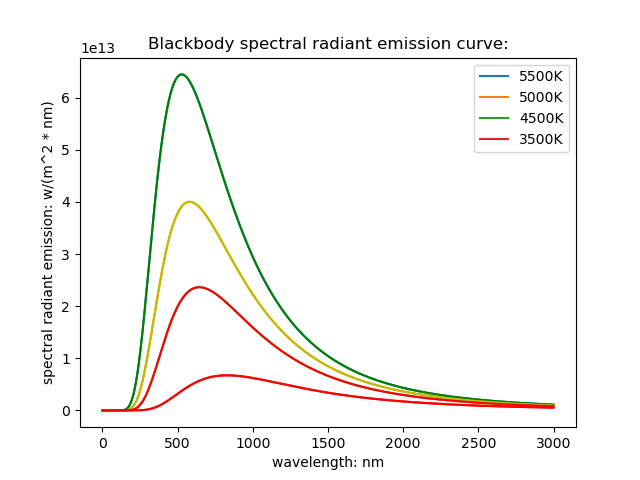
\includegraphics[width=8cm]{Figure_1.png}
	\caption{plank's figure}
\end{figure}
\begin{figure}[H]
	\centering
	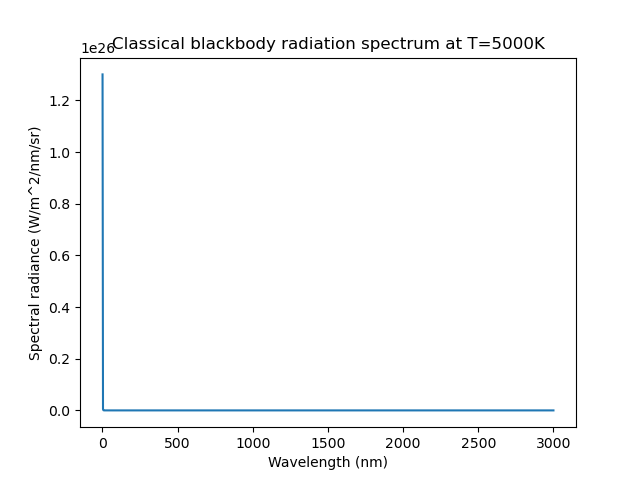
\includegraphics[width=8cm]{Figure_2.png}
	\caption{classical's figure}
\end{figure}

\section[short]{解释}

经典理论和量子理论的结果之间的差异在于:\\

1.经典理论无法解释光子数的量子性质,即经典理论中不存在能量的量子化,因此无法描述光的离散性质。而量子理论则将光看作一组离散的光子,每个光子都有确定的能量和动量。\\

2.在经典理论中,黑体辐射的能量密度随着频率的增加而无限增大,这与实验结果不符。而量子理论中,能量密度随着频率的增加呈现峰值,并随着温度的升高而整体上升。\\

3.经典理论无法解释热容量的温度依赖性,即热容量随着温度的升高而增加,而在量子理论中,热容量随着温度的升高呈现先增加后减少的曲线。\\

因此,量子理论与经典理论的差异在于量子理论具有量子化的性质,并且可以解释实验结果,而经典理论则无法完全解释黑体辐射的行为。\\


根据光谱图形来看(图3),经典理论的结果会产生紫外灾变,即预测在短波长处出现的强烈辐射,这与实验观测到的黑体辐射谱并不符合。
而量子理论给出的结果则可以很好地解释黑体辐射谱的整体形状,特别是在短波长和长波长端的行为,符合实验观测。

\begin{figure}[H]
	\centering
	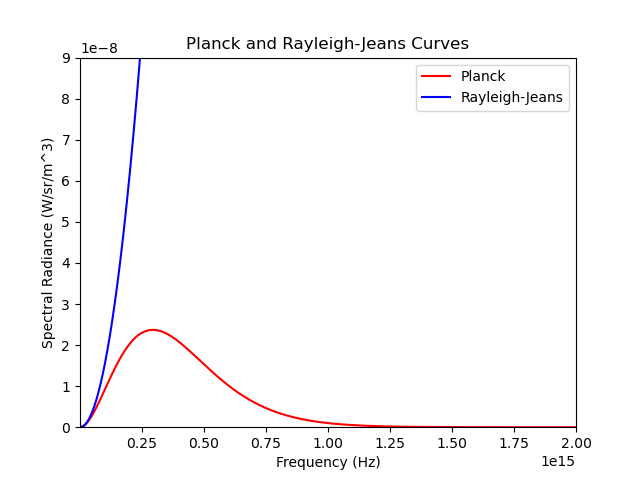
\includegraphics[width=8cm]{Figure_3 freq.png}
	\caption{可以看出他们之间相差非常大}
\end{figure}
\section{Code}

\begin{lstlisting}[language=Python, caption=planck]
    import numpy as np 
    import matplotlib.pyplot as plt 
    
    
    def planck(wavelength,temperature):
        c1=3.746*10**(-16)
        c2=1.4404*10**(-2)
        return (c1/(wavelength**5))*(1/(np.e**(c2/(wavelength*temperature))-1))
    
    wavelengths = np.arange(1e-9, 3e-6, 1e-9)
    out_5500 = planck(wavelengths,5500)
    out_5000 = planck(wavelengths,5000)
    out_4500 = planck(wavelengths,4500)
    out_3500 = planck(wavelengths,3500)
    
    plot_5500 = plt.plot(wavelengths*10**9,out_4000,label='5500K')
    plot_5000 = plt.plot(wavelengths*10**9,out_5000,label='5000K')
    plot_4500 = plt.plot(wavelengths*10**9,out_6000,label='4500K')
    plot_3500 = plt.plot(wavelengths*10**9,out_7000,label='3500K')
    
    
    
    plt.plot(wavelengths*1e9, out_5500, 'g-')
    plt.plot(wavelengths*1e9, out_5000, 'y-')
    plt.plot(wavelengths*1e9, out_4500, 'r-')
    plt.plot(wavelengths*1e9, out_3500, 'r-')
    
    plt.xlabel('wavelength: nm')
    plt.ylabel('spectral radiant emission: w/(m^2 * nm)')
    plt.title('Blackbody spectral radiant emission curve:')
    plt.legend()
    plt.show()
    
    
\end{lstlisting}
\begin{lstlisting}[language=Python, caption=classical]
    import numpy as np
    import matplotlib.pyplot as plt

    h = 6.626e-34    
    c = 2.998e8      
    k = 1.381e-23    
    T = 5000         
    wavelengths = np.linspace(1e-9, 3e-6, 1000)

    I_lambda = 2 * np.pi * k * T * c / wavelengths**4

    plt.plot(wavelengths * 1e9, I_lambda)
    plt.xlabel('Wavelength (nm)')
    plt.ylabel('Spectral radiance (W/m^2/nm/sr)')
    plt.title('Classical blackbody radiation spectrum at T=5000K')
    plt.show()

\end{lstlisting}

\begin{lstlisting}[language=Python, caption=comparision]
    import numpy as np
    import matplotlib.pyplot as plt


    h = 6.62607015e-34
    c = 2.99792458e8
    k = 1.380649e-23


    def Planck(x, T):
        return (2 * h * c ** 2 / (x ** 5)) * (1 / (np.exp(h * c / (x * k * T)) - 1))

    def RayleighJeans(x, T):
        return (8 * np.pi * k * T / (x ** 4))


    T = 5000 
    x = np.linspace(1e-9, 3e-6, 1000000)
    y1 = Planck(x, T)
    y2 = RayleighJeans(x, T) 

   
    fig, ax = plt.subplots()
    ax.plot(x, y1, 'r-', label='Planck')
    ax.plot(x, y2, 'b-', label='Rayleigh-Jeans')
    ax.legend(loc='upper right')
    ax.set_xlabel('Wavelength (m)')
    ax.set_ylabel('Spectral Radiance (W/sr/m^3)')
    ax.set_title('Planck and Rayleigh-Jeans Curves')
    ax.set_xlim([0, 3e-6]) 
    ax.set_ylim([0, 3e15]) 
    plt.show()

\end{lstlisting}

\end{spacing}{}

\bibliographystyle{IEEEtran}
\bibliography{lecktion0}

\end{document}